\section{Test01: GPU vs CPU}
The results of this test are used as baseline for further optimizations. \\
Test configuration:
\begin{itemize}
  \item \textbf{CPU}: Intel(R) Core(TM) i7-4770K CPU @ 3.50GHz 
  \item \textbf{GPU}: NVIDIA Tesla K40c 
\end{itemize}
Implementations tested:
\begin{itemize}
  \item \textbf{legacy\_multifit\_cpu}: plain \textit{cms-sw} cpu code.
  \item \textbf{legacy\_multifit\_gpu}: plain gpu porting \textit{cms-sw} cpu code.
  \item \textbf{multifit\_cpu}: inplace fnnls cpu implementation.
  \item \textbf{multifit\_gpu}: inplace fnnls gpu implementation.
  \item \textbf{multifit\_cpu\_swap}: fnnls cpu implementation with swapping matrices.
  \item \textbf{multifit\_gpu\_swap}: fnnls gpu implementation with swapping matrices.
\end{itemize}
\begin{figure}[h]
  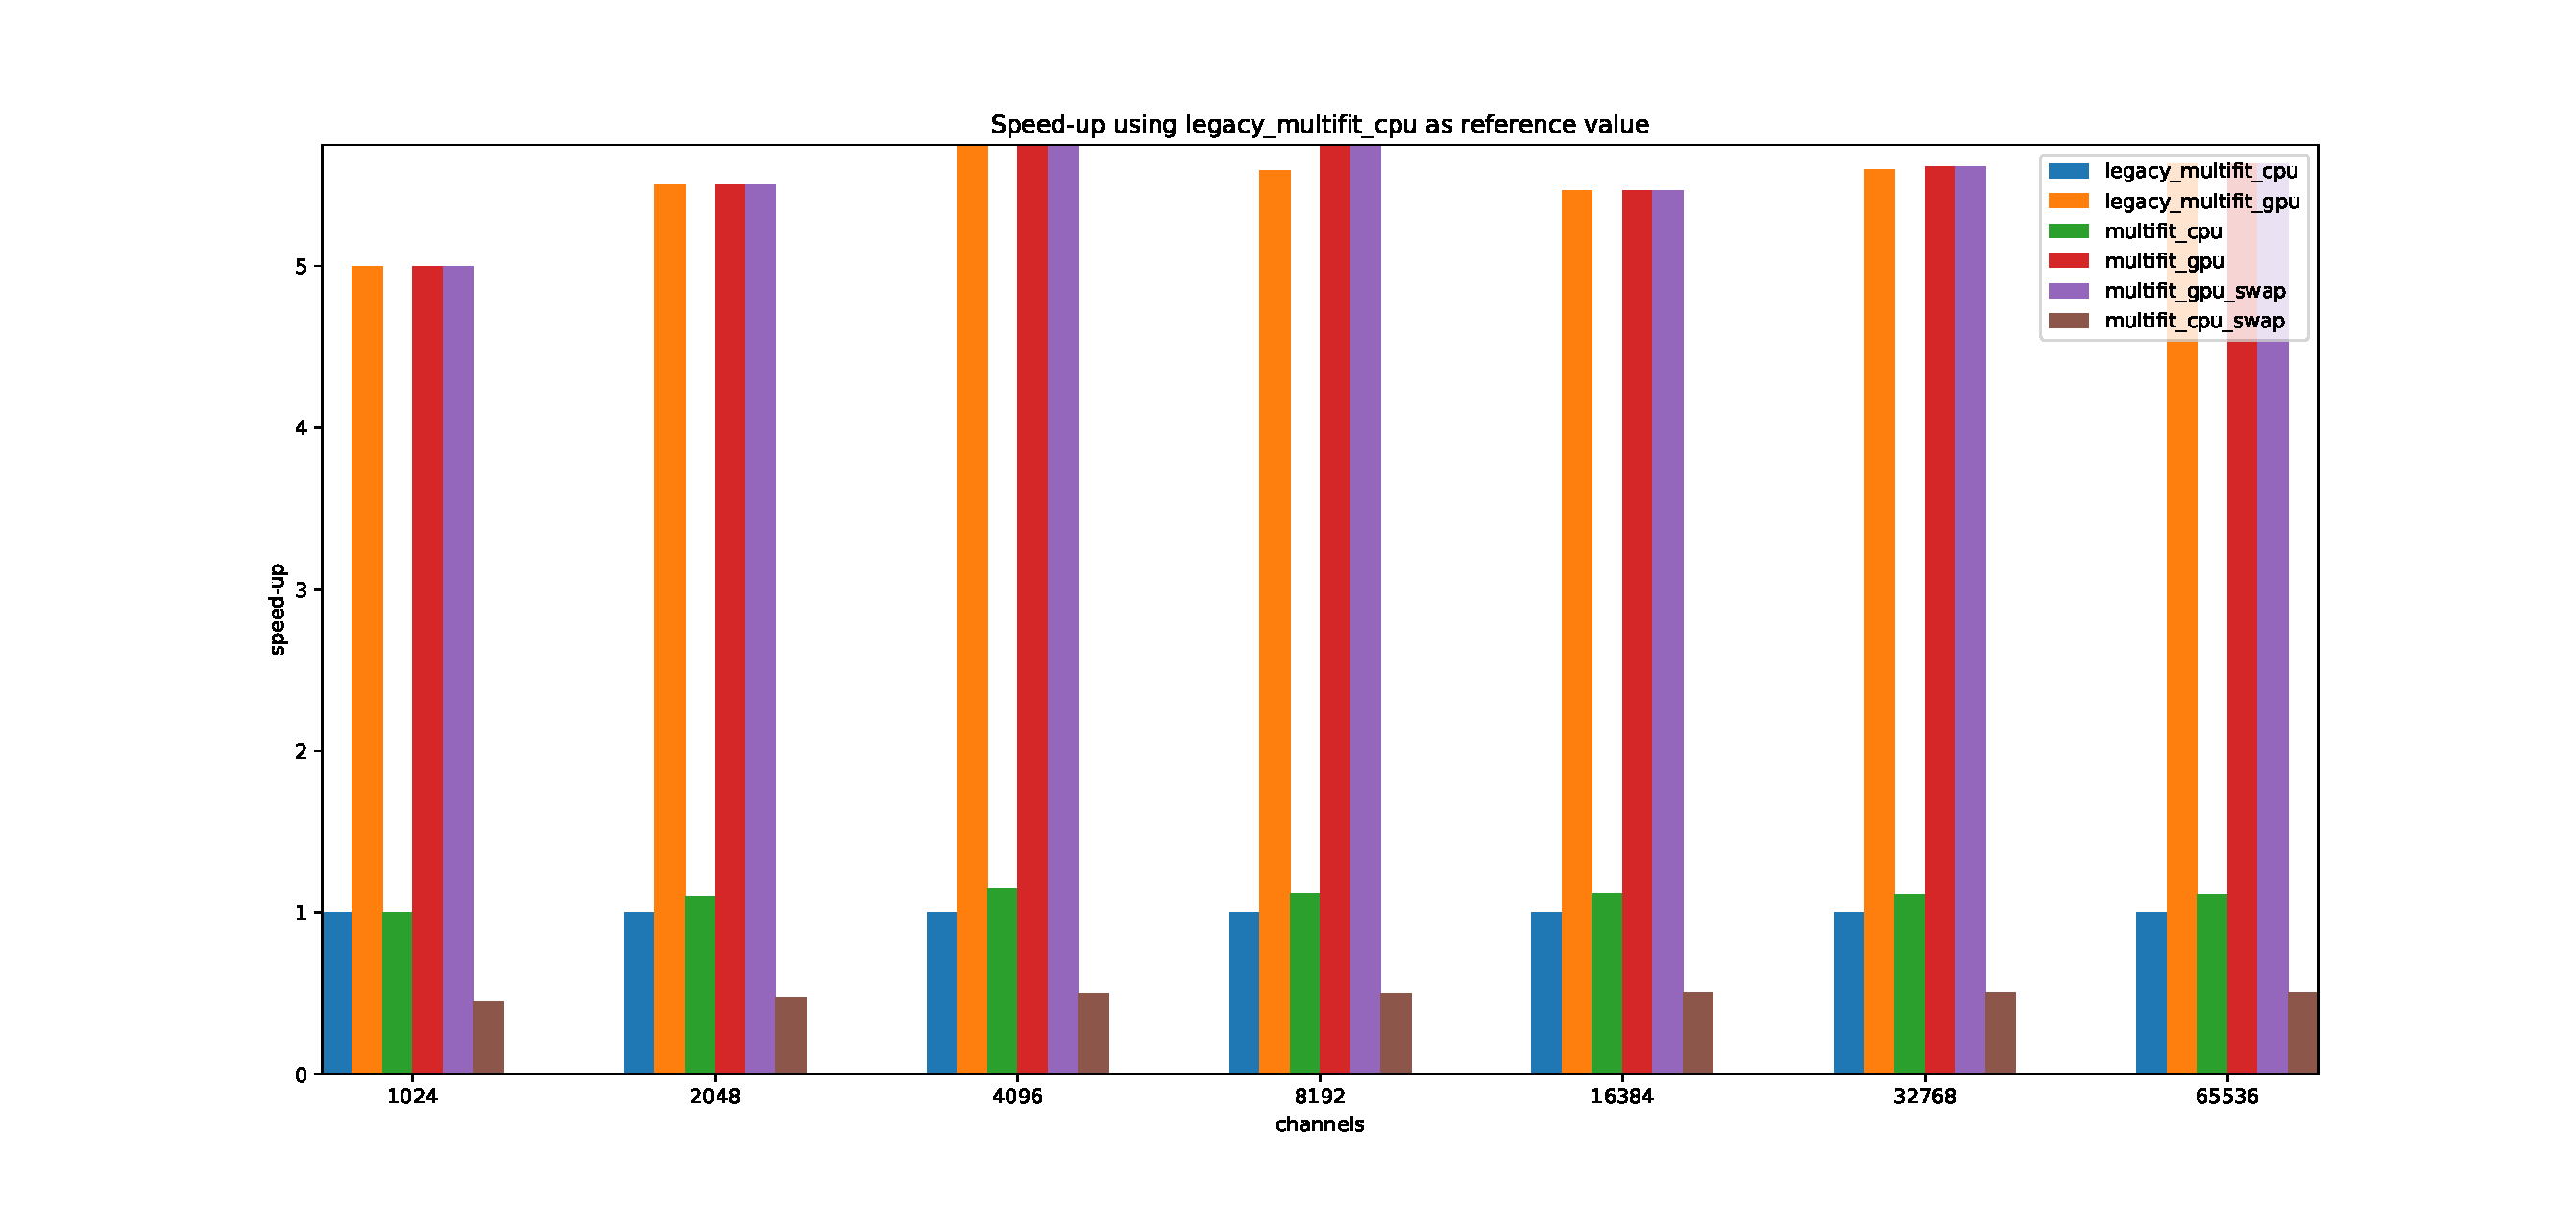
\includegraphics[width=\textwidth]{img/speedup}
  \caption{Speedup achieved with 10 iterations, higher is better}
  \label{img:speedup01}
\end{figure}
All the cpu implementations are single-threaded. With 64k channels the GPU version achieves a speedup of 2.6. 
\begin{figure}[H]
  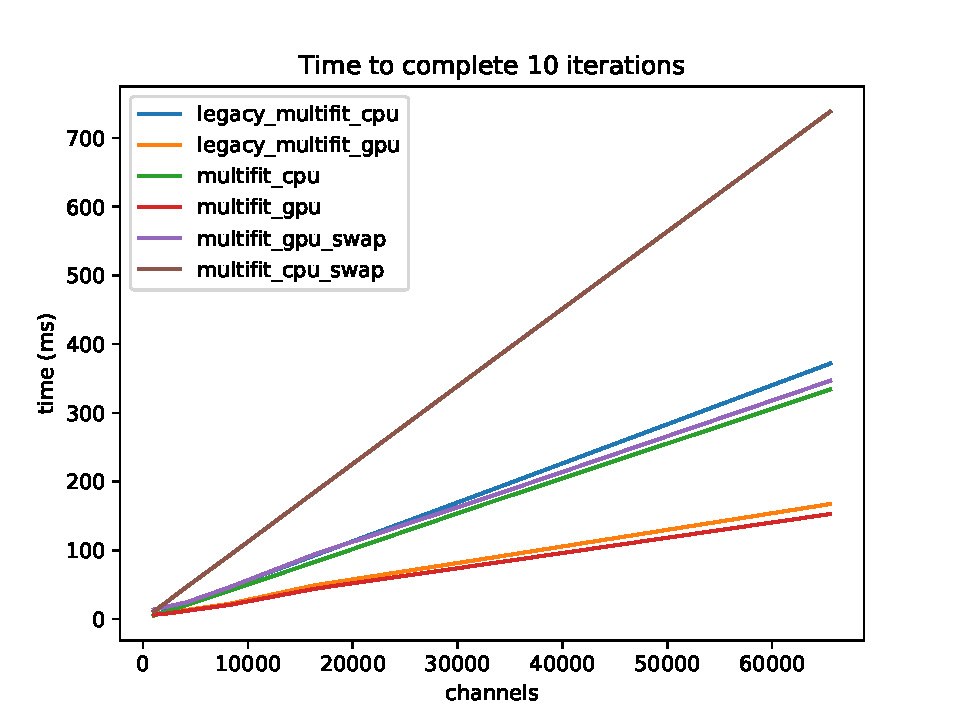
\includegraphics[width=.75\textwidth]{img/linscale}
  \caption{Time needed to complete 10 iterations, linear channel scale, lower is better}
  \label{img:linscale01}
\end{figure}
From \ref{img:speedup01} can be noted that the numerical optimizations allows to achieve a factor of 2 in speedup. The GPU performs twice as fast with respect to the CPU. Other optimizations like loop unrolling and branch reduction give a performance gain about 20\% in CPU and 30\% on GPU.  
\begin{figure}[H]
  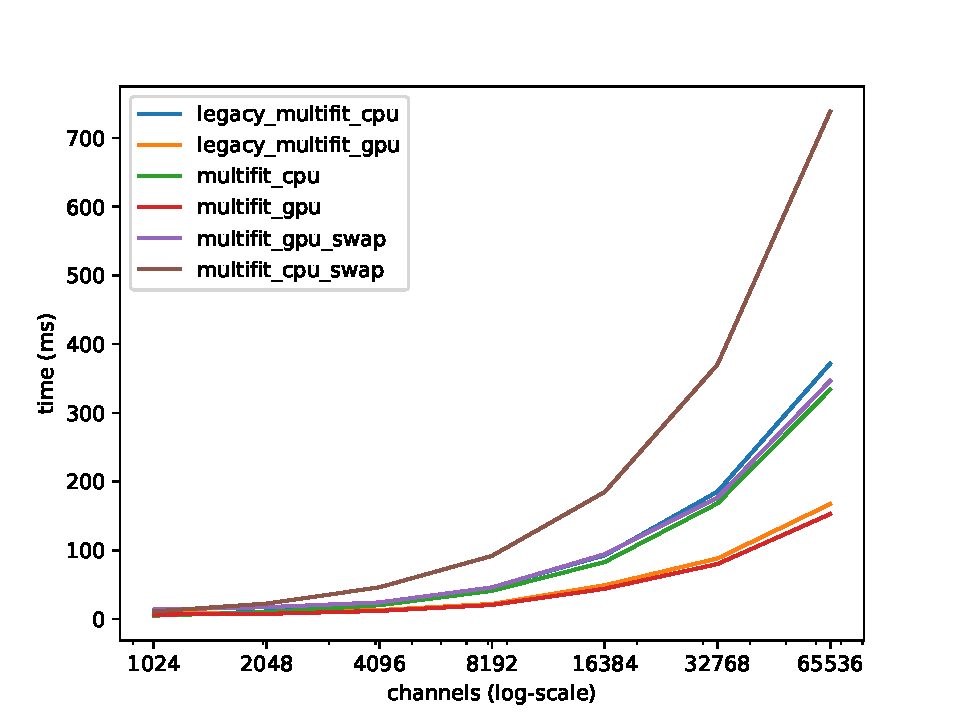
\includegraphics[width=.75\textwidth]{img/logscale}
  \caption{Time needed to complete 10 iterations, log channel scale, lower is better}
  \label{img:logscale01}
\end{figure}
From the plot present in \ref{img:linscale01} can be noted that, on GPU, the time increases faster at the beginning and around 15000 channels there is a change of slope and the increase becomes sub-linear. On the CPU, the increase is linear with respect to the channels.
The plot in \ref{img:logscale01} makes more evident the difference between the different version of the algorithm. The GPU outperforms the CPU and it will be interesting to study what will happen if the number of channels increases even more.\\

